\chapter{Конструкторская часть}

В данном разделе будут рассмотрены схемы описанных в предыдущем разделе алгоритмов сортировок.

На рисунке \ref{fig:insertion} приведена схема алгоритма сортировки вставками.

\begin{figure}[h!]
	
	\centering{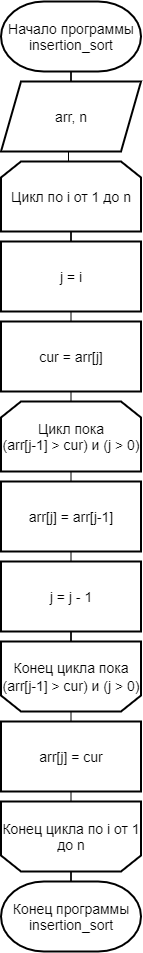
\includegraphics[scale=0.5]{inc/img/insertion.png}}
	
	\caption{Схема алгоритма сортировки вставками}
	
	\label{fig:insertion}
	
\end{figure}


На рисунке \ref{fig:bubble} приведена схема алгоритма сортировки пузырьком.

\begin{figure}[h!]
	
	\centering{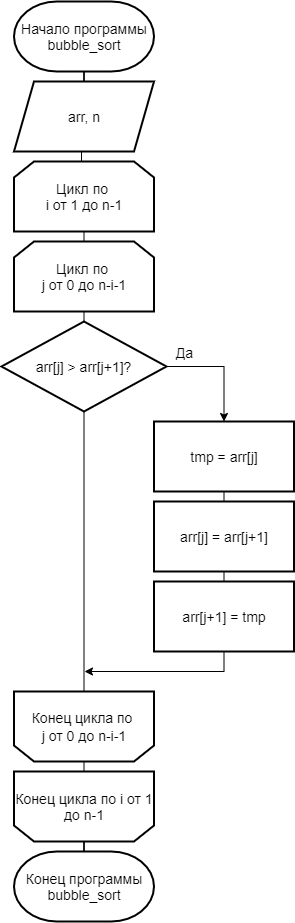
\includegraphics[scale=0.5]{inc/img/bubble.png}}
	
	\caption{Схема алгоритма сортировки пузырьком}
	
	\label{fig:bubble}
	
\end{figure}

На рисунке \ref{fig:shaker} приведена схема алгоритма шейкерной сортировки.

\begin{figure}[h!]
	
	\centering{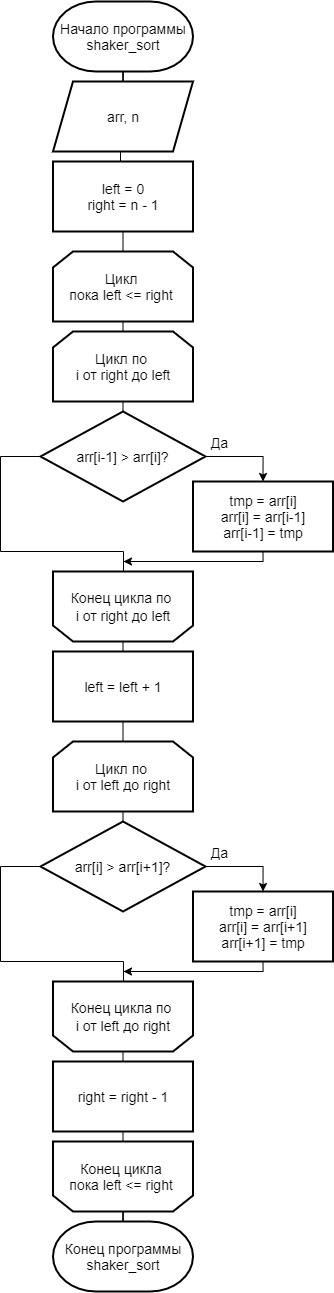
\includegraphics[scale=0.5]{inc/img/shaker.png}}
	
	\caption{Схема алгоритма шейкерной сортировки}
	
	\label{fig:shaker}
	
\end{figure}



\section*{Вывод}

Были разработаны схемы трех алгоритмов сортировки.


